\chapter[Product]{Design and Implementation}
\label{design}

	\section{Introduction}
	\label{design:intro}

		Due to the room for research available in this area, it made sense to focus this study on a relatively broad area of the subject to be used as a foundation, rather than to specialise on a particular niche.
		% REWORD THIS?
		Because of this, the main focus for this study is the effects that Non-Euclidean geometry has on a user's sense of Immersion, and to find any changes in a user's comfort navigating in a virtual environment.

		This chapter covers the development process that was undertaken for the creation of the product used for the experiments.

	\section{Development Process}
	\label{design:dev}

		% THIS section will cover the development process of the product itself

		% Talk about development methodologies considered for use with the project, and how they were adapted for use for a single person.
			% Use of Git and stuff like that

		% Talk about how you decide to use an existing engine you knew well (save time reinventing the wheel for things like lighting, camera stuff, etc)
		% Also you wanted to limit the amount of outside variables as possible, so an existing engine helped with that

		% Talk about implementation process
			% Started off using render textures, but that had problems regarding depth perception, outside of VR it was fine but inside it was obviously a plane
			% Changed to using render culling and directly viewing the cameras with a bit more tranlation and rotation magics
			% Challenge with multiple variations in how the areas can be set up - angles, inversions on both sides, whether one or both should render, whether you should be able to use it to transport, etc


	\section{Product model}
	\label{design:model}

		% THIS section will contain models of the various states and relations between the functions and other workings of the product, for areas such as the transition between non-Euclidean world areas.
		\autoref{appendix:code:camera} \autoref{appendix:code:player}

	\begin{figure}[H]
		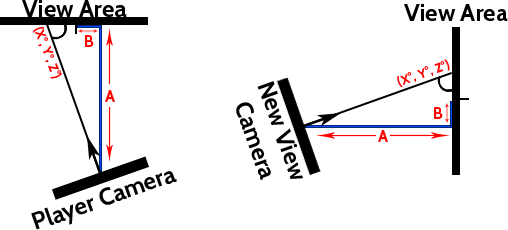
\includegraphics[width=0.8\textwidth]{Images/Position}
		\centering
		\caption{2D representation of the calculations for the position and rotation of cameras.
			See \autoref{appendix:code:camera} for the implementation}
		\label{design:fig:maths}
	\end{figure}

	\begin{figure}[H]
		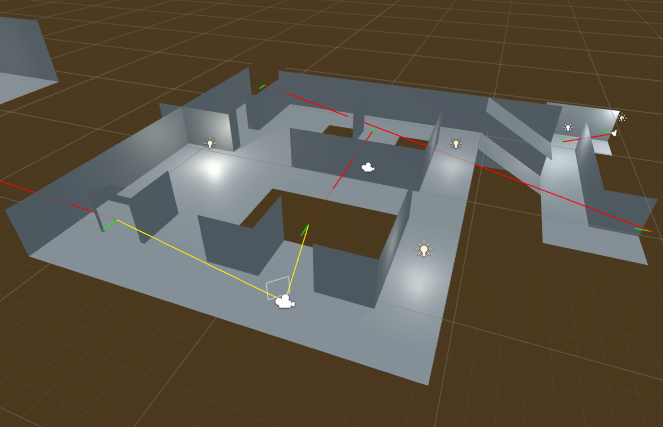
\includegraphics[width=1\textwidth]{Images/Lines_Everywhere2}
		\centering
		\caption{Example view of a scene.
			Red lines are connections between points,
			yellow lines are connections visible to the player,
			and green lines are the direction the connectors are facing}
		\label{design:fig:scene}
	\end{figure}

	\begin{figure}[H]
		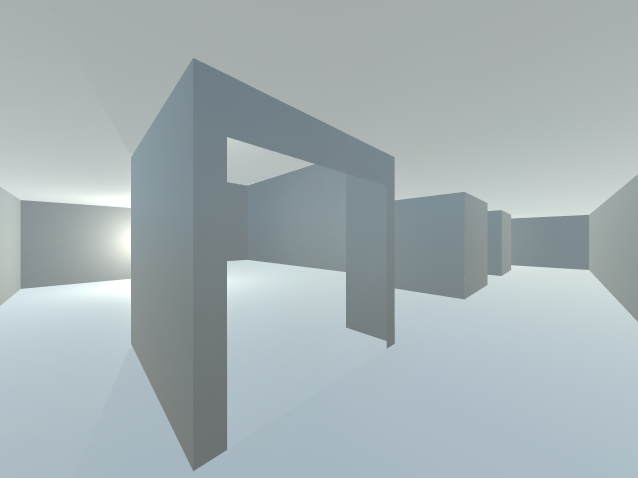
\includegraphics[width=1\textwidth]{Images/NE_View}
		\centering
		\caption{Example of view from inside the Non-Euclidean scene, displaying an area which is larger on the inside}
		\label{design:fig:game}
	\end{figure}

	\section[Environment Design]{Design of experiment environments}
	\label{design:design}

		The design of the environments to be used in the experiments is almost as important as the functionality of the system itself, as it is the only medium through which the participants will be able to provide feedback.
		Two separate scenes were created for use in the experiments, one where the participants would be navigating through a non-Euclidean environment, and the other which would only make use of standard Euclidean space. % TODO: Reword this?

		To limit the number of factors which could affect the immersion of a participant in the experiments, a minimalistic aesthetic was chosen for the scenes.
		By using simple white texturing and relying on lighting for definition, impurities that could be noticed by pixelation of detailed textures were removed, focusing the participant's attention solely on the geometry of the scenes.
		Similarly, the scenes themselves were modelled using simple primitive shapes, such as planes and cubes, to try and minimise any impacts in immersion that could be caused by low polygon counts in more complex models.

		\subsubsection{Non-Euclidean Scene}

			The non-Euclidean test scene (as seen in \autoref{design:fig:design:ne}) was the first of the two scenes to be designed for the experiments.
			As a way to ensure the participants could experience a variety of the possibilities of non-Euclidean environments, a mixture of effects were chosen to be included in the scene, as labelled in \autoref{design:fig:design:ne} by the letters and corresponding red lines.

			\begin{figure}[h]
				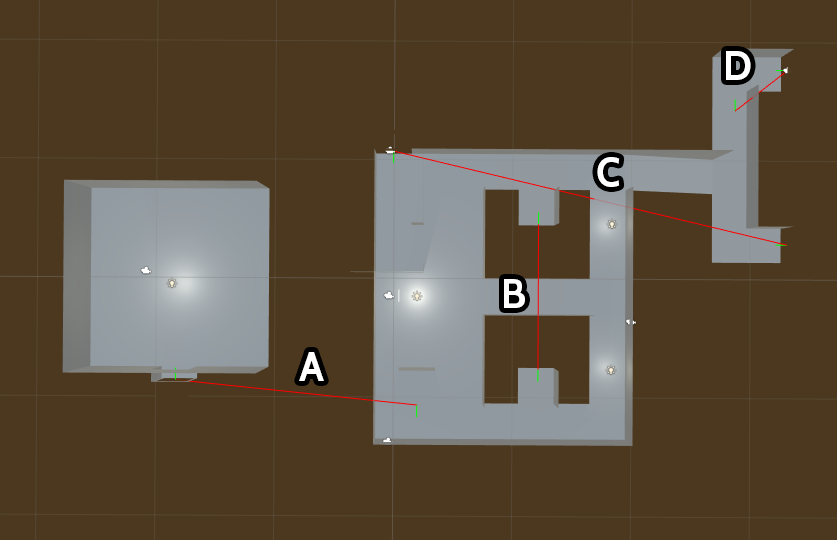
\includegraphics[width=1\textwidth]{Images/NE_Layout}
				\centering
				\caption{Labelled layout of the Non-Euclidean experiment scene}
				\label{design:fig:design:ne}
			\end{figure}

			Point \enquote{A} represents the connection shown in \autoref{design:fig:game}, which is an example of an area appearing to contain a larger area than expected from its surroundings.
			Connection \enquote{B} represents what appears to be a direct corridor to a user which both takes a shorter path than would be expected by the two parallel paths, but also appears to occupy the same space as another corridor which runs perpendicular to it.
			Connection \enquote{C} appears to a user that they are able to walk directly between two completely separate areas of the room, both of which are on different levels (Note the corridor to the right of the \enquote{C} marker is a ramp leading down towards \enquote{D}).
			Finally, connection \enquote{D} gives the impression that the user is walking around a seemingly endless series of turns, however when the user turns back from where they came from, they find they have not travelled anywhere.

		\subsubsection{Standard Scene}
			The standard Euclidean scene (as seen in \autoref{design:fig:design:standard}) was designed to follow a similar layout to the non-Euclidean one, or as close as could be possible with the geometric constraints.
			This decision was made to attempt to limit the factors that could affect the participant's immersion within the scenes, as a way to ensure that the results from the experiments are as consistent as possible.

			\begin{figure}[H]
				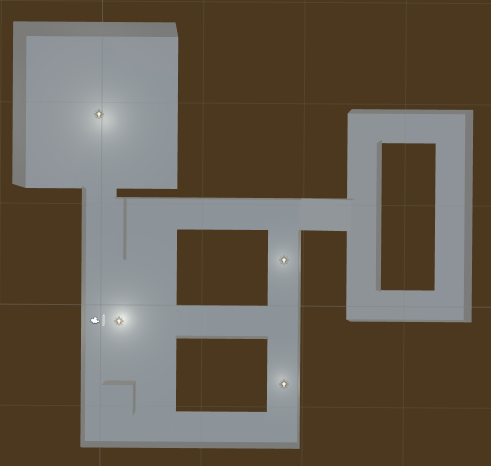
\includegraphics[width=0.7\textwidth]{Images/Standard_Layout}
				\centering
				\caption{Layout of the standard Euclidean experiment scene}
				\label{design:fig:design:standard}
			\end{figure}
